% 5ARE0 Assignment 1 — report starter (NOT a completed assignment report)
% Reconcile final submission ZIP filename with latest Canvas instruction.
\documentclass[10pt,a4paper]{article}
\usepackage[T1]{fontenc}
\usepackage[utf8]{inputenc}
\usepackage{lmodern}
\usepackage[margin=18mm,headheight=13pt]{geometry}
\usepackage{microtype}
\usepackage{graphicx}
\usepackage{booktabs}
\usepackage{tabularx}
\usepackage{array}
\usepackage{amsmath}
\usepackage{enumitem}
\usepackage{xcolor}
\usepackage{hyperref}
\usepackage[backend=biber,style=numeric,sorting=none]{biblatex}
\usepackage[toc,page]{appendix}
\usepackage{etoolbox}

\addbibresource{references.bib}
\hypersetup{colorlinks=true,urlcolor=blue!50!black,linkcolor=black,citecolor=blue!50!black}
\setlength{\parindent}{0pt}
\setlength{\parskip}{4pt}
\setlist[itemize]{nosep,leftmargin=1.3em}
\setlist[enumerate]{nosep,leftmargin=1.3em}
\newcommand{\fillme}[1]{\textcolor{gray}{\textit{[Insert: #1]}}}
\newcommand{\figorplaceholder}[4]{%
  \begin{figure}[htbp]
  \centering
  \IfFileExists{#1}{\includegraphics[width=#2\linewidth]{#1}}{\fbox{\parbox[c][16mm][c]{0.88\linewidth}{\centering\small\fillme{Place figure at \texttt{\detokenize{#1}}}}}}%
  \caption{#3}\label{#4}
  \end{figure}%
}

\begin{document}
\begin{center}
 {\large\bfseries Assessing Bicycle Lane Quality Using Smartphone Sensor Data}\\[3pt]
 {\bfseries 5ARE0 — Data Analysis \& Learning Methods | Assignment 1 | Group 5}\\[4pt]
 Su Acar (2475901) \quad Vikram Chandrasekaran (2542544)\\
 Henrique DaSilva Couto (2463334)\\[3pt]
 \today
\end{center}
\vspace{-5pt}\hrule\vspace{4pt}
\small
% Up to 8 pages according to the assignment PDF. Keep this heading compact.
% Replace every [Insert: ...] placeholder with your group's own analysis and verified results.
\section{Introduction}
The CRISP-DM (CRoss-Industry Standard Process for Data Mining) framework described by \cite{shearer00crisp} was used as the underlying framework for structuring the project and report. The CRISP-DM framework consists of six phases: Business Understanding, Data Understanding, Data Preparation, Modeling, Evaluation and Deployment. The following sections of this report are structured according to these phases.

The group adopted an experimental approach to investigate the data and establish frequencies of interest related to the type of road. The empirical hypothesis was that a so-called 'bumpy' road would, by definition, present a higher energy in the band of interest due to vertical vibration, which is basically the rider's perceived shaking experience when cycling through a bumpy versus a smooth path.

\fbox{%
  \parbox{1.0\textwidth}{%
    \textbf{\underline{Technology Statement}}: During the preparation of this work, we used OpenAI ChatGPT (GPT-5.6 Sol), Google Gemini (3.1 Pro) and Claude Sonnet 5 Medium in order to brainstorm assignment direction, support on coding and discuss specific technical concepts to support the team along the development. The following parts of the assignment were affected/generated by AI tool usage: DATA UNDERSTANDING / DATA PREPARATION / MODELING / EVALUATION / DEPLOYMENT. After using this tool/service, [Su Acar, Vikram Chandrasekaran and Henrique da Silva Couto] evaluated the validity of the tool’s outputs, including the sources that generative AI tools have used, and edited the content as needed. As a consequence, [Su Acar, Vikram Chandrasekaran and Henrique da Silva Couto] take full responsibility for the content of their work.
  }%
}

\section{Business / Objective Understanding}
If a rider could close their eyes while cycling (which is not recommended by obvious reasons), this person's body would be able to clearly feel that they are passing either in a smooth or in a bumpy road. Perhaps one of the easiest ways to explain that in physics-related terms would be that when one is crossing a bumpy path, the dynamic vertical acceleration of one's bicycle is much more noticeable (and uncomfortable) if compared to a completely smooth terrain.

This definition gives us a strong hypothesis to test. If this very distinctive vibration feeling that the riders experiment can be derived from the sensors already present in a smartphone, for instance, that would be a clear and well-defined way to feed an autonomous classifier to ingest and analyse the sensor data, providing a real-time diagnostic whether a bike path is smooth or bumpy.

Naturally, this diagnostic is irrelevant on a user by user basis. As we already established, it's quite easy to feel the condition of the road you are cycling in. Accordingly, the value of such a classifier would be perceived for stakeholders responsible for providing adequate road conditions, or even more so, to equip the community with a tool to evaluate which parts of a given municipality need smoother cycling paths.

Considering the actual classifier, what is important to determine and establish in terms of scope is the ability of the model to separate between two distinct classes: \textit{smooth} and \textit{bumpy}. So, let's define that a single pothole in a smooth bicycle lane \textbf{should not} necessarily trigger a bumpy classification. As much as a pothole needs fixing to avoid accidents, this should fall in routine repairs and, as stated, the objective here is to raise awareness to bumpy lanes that need to be, at some point, converted to smooth ones.

\textbf{Research objective.}
As a high level model design criteria, the targets were defined as: $"Smooth" = 0$ and $"Bumpy" = 1$. Since the main objective is to locate paths which are bumpy across cities and villages, what is most important for this model is to avoid classifying smooth roads as bumpy, in other words, we need a model focused on delivering $\text{high precision}$ bumpy outcomes, supported by a low $\frac{\text{false positive rate}}{specificity}$, where a false positive is defined as: $\text{actual Smooth → predicted Bumpy}$.
\begin{itemize}
    \item headline metric      = Bumpy precision
    \item direct FP metric     = Smooth specificity / false-positive rate
    \item anti-degenerate check = Bumpy recall + F0.5
\end{itemize}

It is important to notice that we should not optimise precision alone and then hide recall. A model that would never predict `Bumpy`can obtain excellent precision, while being useless in practice.

\fbox{%
  \parbox{1.0\textwidth}{%
    \textbf{\underline{Technology Statement}}: During the preparation of this work, we used OpenAI ChatGPT (GPT-5.6 Sol), Google Gemini (3.1 Pro) and Claude Sonnet 5 Medium in order to brainstorm assignment direction, support on coding and discuss specific technical concepts to support the team along the development. The following parts of the assignment were affected/generated by AI tool usage: [DATA PREPARATION / MODELING / EVALUATION]. After using this tool/service, [Su Acar, Vikram Chandrasekaran and Henrique da Silva Couto] evaluated the validity of the tool’s outputs, including the sources that generative AI tools have used, and edited the content as needed. As a consequence, [Su Acar, Vikram Chandrasekaran and Henrique da Silva Couto] take full responsibility for the content of their work.
  }%
}

\section{Data Understanding}
\textbf{Acquisition protocol.} \fillme{Participants, anonymization, back-pocket placement, accelerometer/gravity/gyroscope configuration, number/duration/terrain of rides, and source organization.}

\textbf{Quality screening.} \fillme{Show measured sampling rates; document exclusion of participant \#03 (~62 Hz, Nyquist ~31 Hz, incompatible with 40--46 Hz features). Describe what this does to participant generalizability.}

\textbf{Available independent units.} \fillme{State both number of windows and independent original recording/session groups; identify how Raw031--Raw041 map to two parent sessions.}

\subsection{Empirical Measurements - Road Frequency versus Leg Movement Artifacts}
It was decided to conduct an experiment to evaluate whether there was a possible overlap with low frequency artifacts (such as leg movements) with the natural vibration caused by the gaps on the road.

Accordingly, an empirical experiment was carried out to empirically measure those frequencies.

\begin{figure}[htbp]
    \centering
    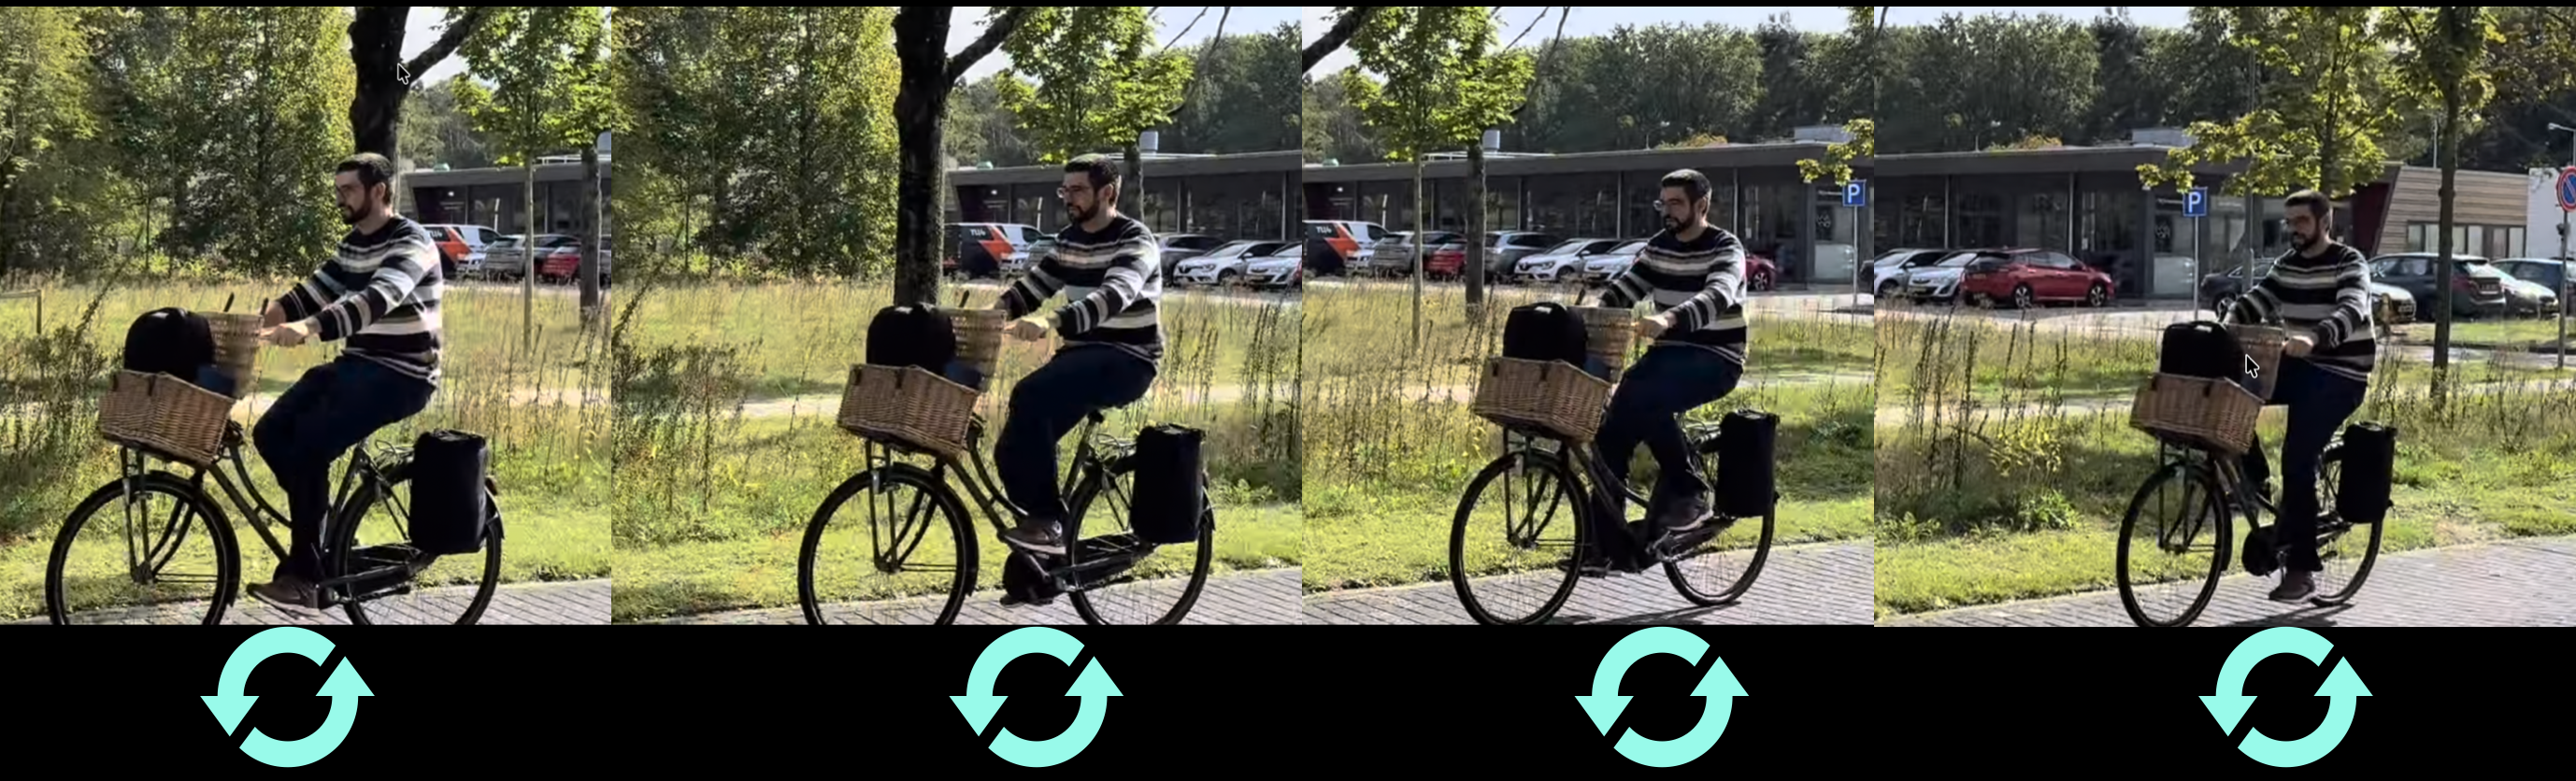
\includegraphics[width=0.8\linewidth]{figures/leg-movement}
    \caption{Example of manually counting the rotations per minute based on the video recording from one of the participants.}
    \label{fig:leg-mov}
\end{figure}

\begin{figure}[htbp]
    \centering
    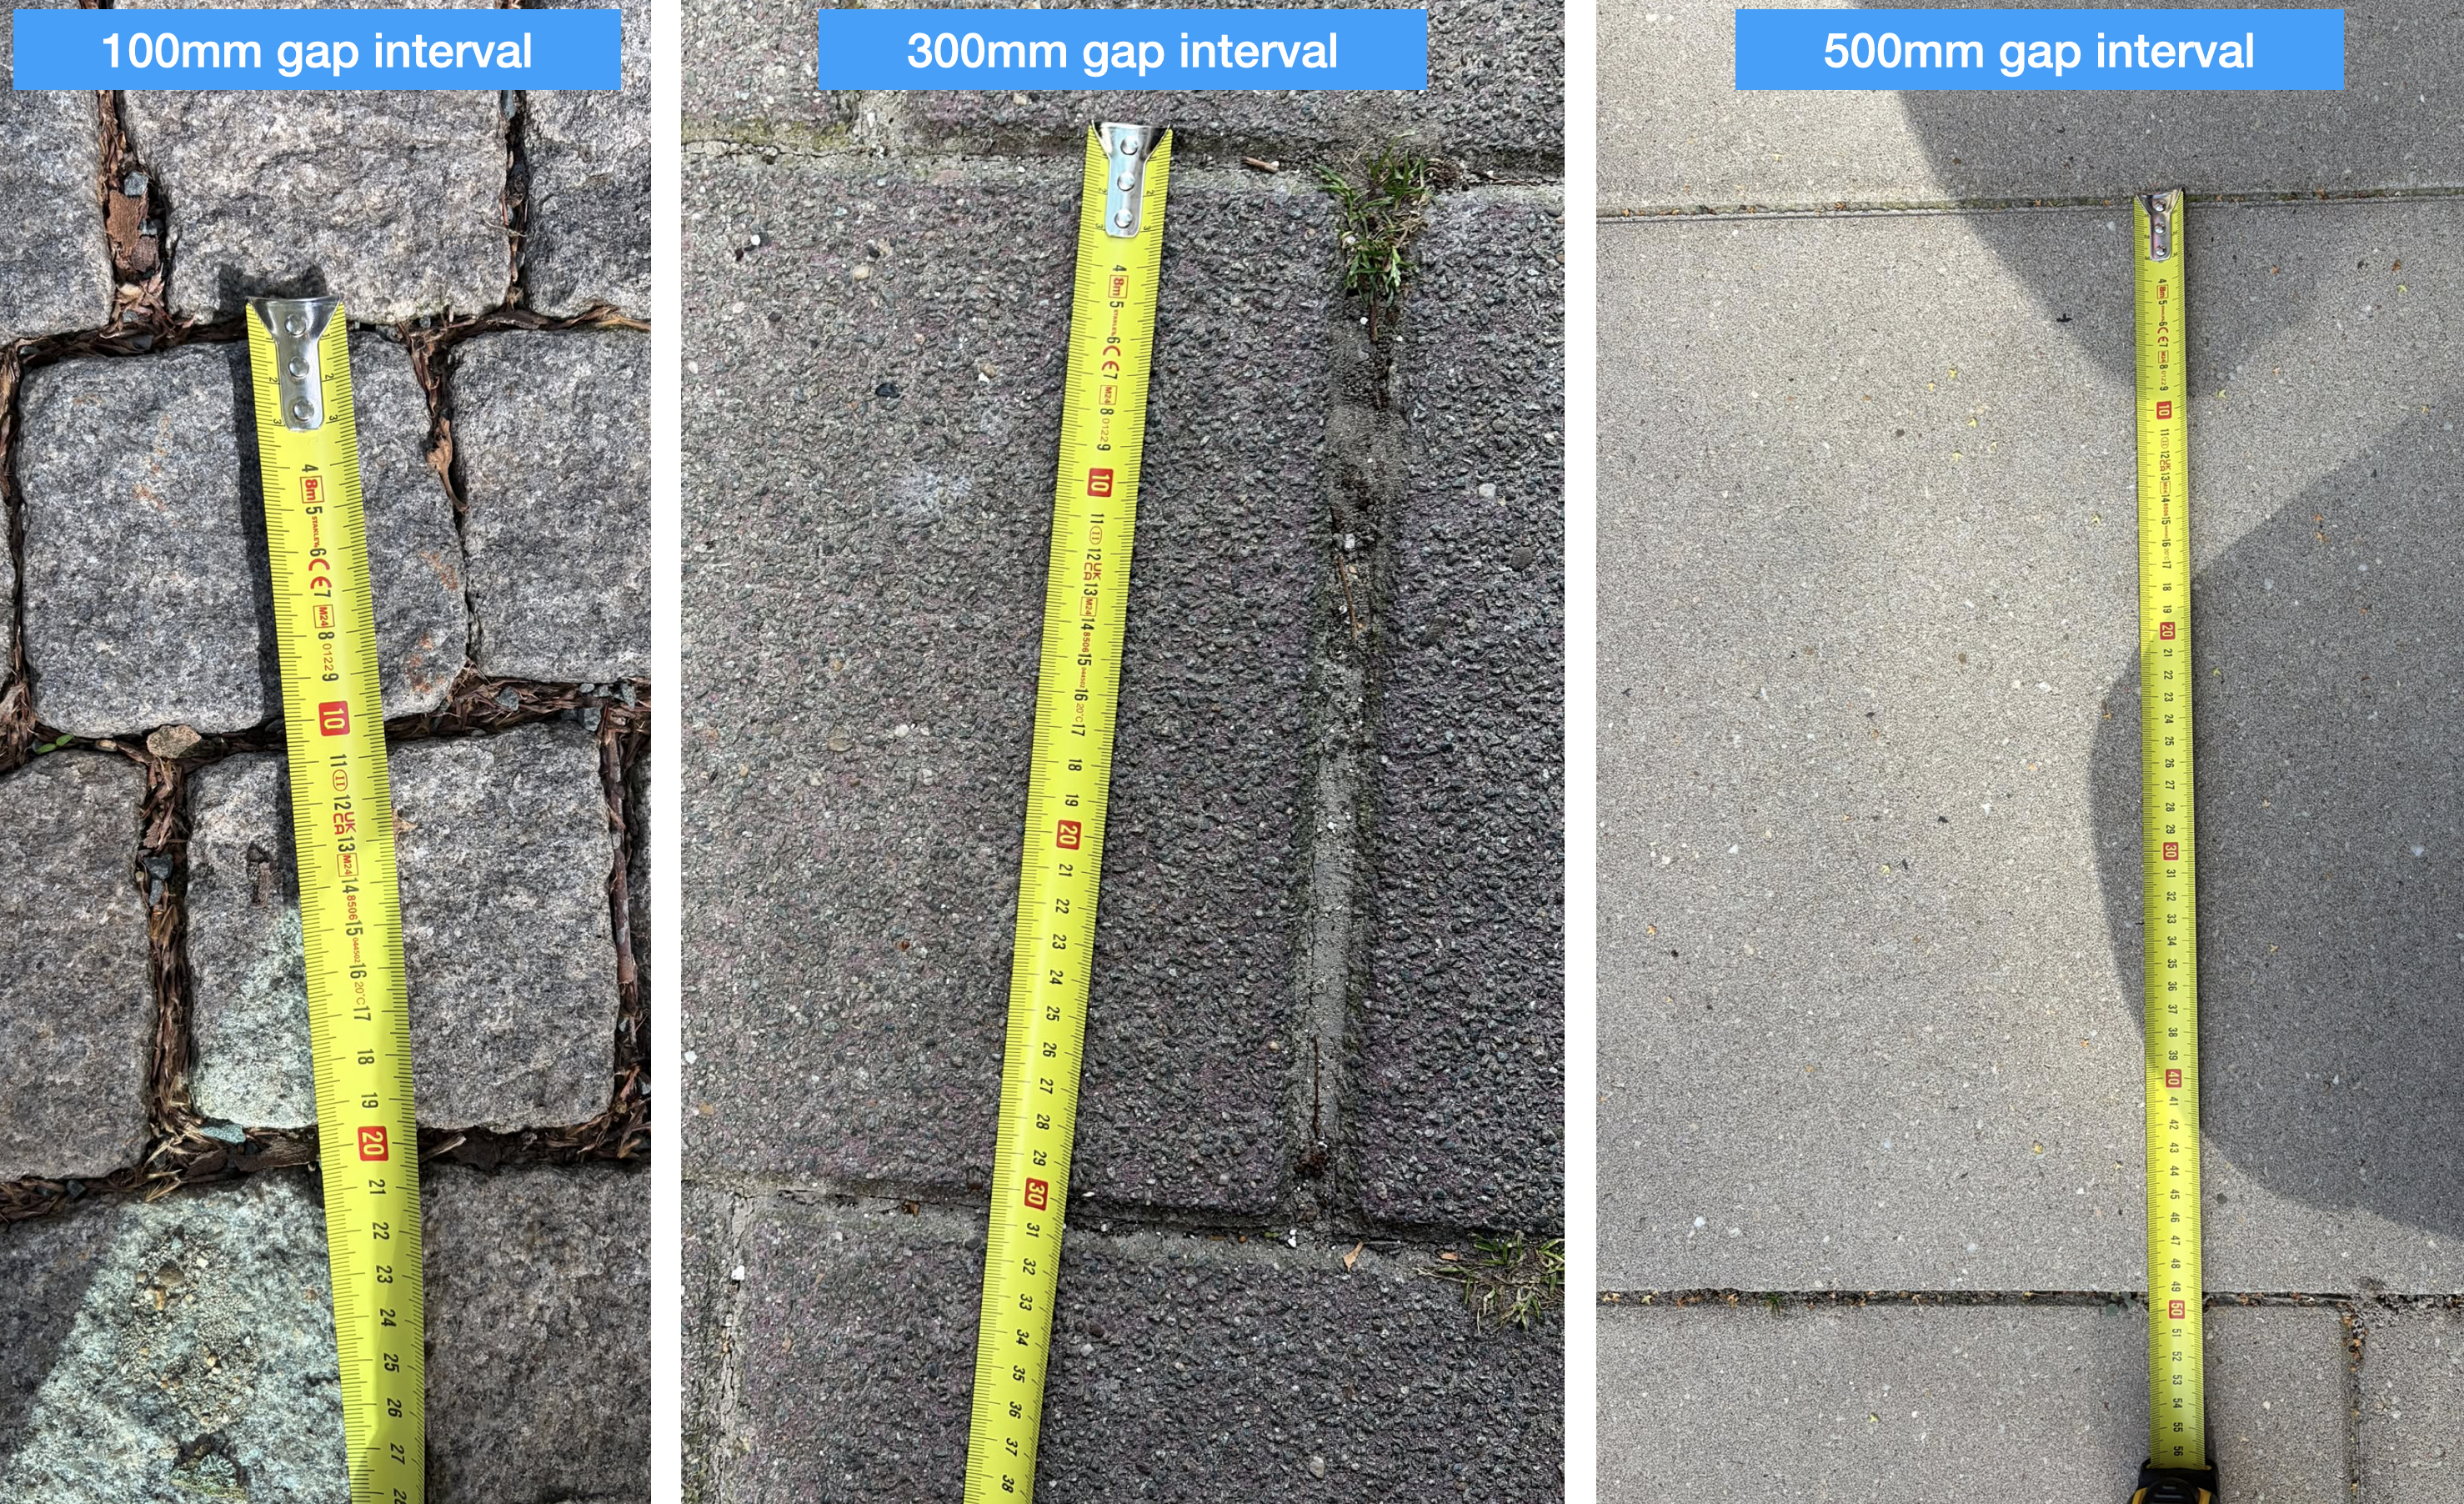
\includegraphics[width=0.8\linewidth]{figures/gap-bumpy-terrain}
    \caption{Different types of bumpy terrains were considered. The measured terrains ranged from $100 \sim 500mm$ gap interval.}
    \label{fig:road-gaps}
\end{figure}


The approximate road-excitation frequency was estimated from the measured
cycling velocity and the spatial spacing between terrain irregularities:

\begin{equation}
    f_{\text{road}} \approx \frac{v}{\lambda},
\end{equation}

where $v$ is the bicycle velocity and $\lambda$ is the spatial terrain
spacing. For the experiment, $\lambda = 100$ mm $= 0.1$ m. The bicycle
velocity was calculated from the travelled distance $d$ and the mean time
of the three repetitions:

\begin{equation}
    v = \frac{d}{\bar{t}}.
\end{equation}

Pedalling frequency was estimated by manually counting complete leg-motion
cycles over a measured video duration:

\begin{equation}
    f_{\text{pedal}} = \frac{N_{\text{cycles}}}{t},
\end{equation}

with cadence expressed in revolutions per minute as

\begin{equation}
    \mathrm{RPM} = 60 f_{\text{pedal}}.
\end{equation}

\begin{table}[htbp]
    \centering
    \caption{Measured cycling speed and estimated road-excitation frequency for a terrain spacing of $\lambda = 100$ mm.}
    \label{tab:road_frequency}
    \begin{tabular}{ccccccccc}
        \toprule
        $\lambda$ 
        & Distance
        & Intended
        & $t_1$
        & $t_2$
        & $t_3$
        & $\bar{t}$
        & Speed
        & $f_{\text{road}}$ \\
        (mm)
        & (m)
        & speed
        & (s)
        & (s)
        & (s)
        & (s)
        & (m/s)
        & (Hz) \\
        \midrule
        100 & 10 & Slow   & 3.63 & 4.06 & 4.03 & 3.91 & 2.56 & 25.60 \\
        100 & 10 & Medium & 2.50 & 2.45 & 2.60 & 2.52 & 3.97 & 39.74 \\
        100 & 10 & Fast   & 1.95 & 1.85 & 2.06 & 1.95 & 5.12 & 51.19 \\
        \bottomrule
    \end{tabular}
    \label{tab:road-freq}
\end{table}

As shown in table \ref{tab:road-freq}, the data was calculated for a gap interval $\lambda = 100mm$. As it can be seen in figure \ref{fig:road-gaps}, we can easily extrapolate those results with $\lambda=300mm$ and $\lambda=500mm$.

We already know the higher end of the spectrum, with $\lambda = 100mm$ at maximum speeds, which yields a road frequency of $\approx 51Hz$. To estimate to the best of our abilities the other side of the spectrum, we need to consider the maximum gap measured ($\lambda = 500mm$), associated with the slowest speed in table \ref{tab:road-freq} ($\approx 2.5 m/s$) which will, in turn, result in a minimum road frequency of $\approx 5Hz$.


\begin{table}[htbp]
    \centering
    \caption{Estimated pedalling cadence from manually counted leg-motion cycles.}
    \label{tab:pedalling_frequency}
    \begin{tabular}{lcccc}
        \toprule
        Video
        & Duration
        & Cycles counted
        & $f_{\text{pedal}}$
        & Cadence \\
        & (s)
        &
        & (Hz)
        & (RPM) \\
        \midrule
        rpm-video-1.mp4 & 17 & 26 & 1.53 & 91.76 \\
        rpm-video-2.mp4 & 21 & 30 & 1.43 & 85.71 \\
        rpm-video-3.mp4 & 25 & 30 & 1.20 & 72.00 \\
        \bottomrule
    \end{tabular}
    \label{tab:leg-rpm}
\end{table}

Based on the results computed in table \ref{tab:leg-rpm}, it is clear important to observe that we're only interested in the highest possible speed, and that is why the group participant was request to cycle as fast as possible. Since a single gear bicycle was used in the experiment, one could claim that the number of leg revolutions would be as high as possible and still, the maximum frequency observed was still under $2 Hz$.

The combined results of both experiments offer a solid base for the intuition that there seems to be, indeed, a gap in the frequency spectrum of the leg movements and the road vibration frequency. 



\figorplaceholder{figures/sampling_rates.pdf}{0.76}{Measured sampling-rate checks across the acquired recordings.}{fig:sampling}

\section{Data Preparation}
\textbf{Processing pipeline.} \fillme{Sensor alignment, calibrated dynamic acceleration projected along the gravity direction, gyro magnitude, jerk, operational-state gating and 2 s transition exclusion. Explain that centred filters are offline/noncausal.}

\textbf{Frequency analysis and windowing.} \fillme{State the physics-informed 4--46 Hz Butterworth analysis band, Welch PSD, 2 s windows and 50\% overlap; do not claim everything inside the band is road-caused.}

\textbf{Features and reduction.} \fillme{Document the 12 engineered candidates; correlation and mutual-information analysis using TRAIN only; motivate compact sets and note redundancy/physical interpretation.}

\figorplaceholder{figures/state_gating.pdf}{0.90}{Operational-state gating and valid riding segments.}{fig:gating}
\figorplaceholder{figures/psd_terrain.pdf}{0.82}{State-gated PSD comparison between Smooth and Bumpy windows.}{fig:psd}

\section{Modeling}
\textbf{Partitioning.} \fillme{Describe frozen multi-participant, complete-recording 78/22 hold-out; 13 independent training split groups, including two original parent sessions. Explain grouped internal validation and scaling within each fold.}

\textbf{Candidate feature sets.} \fillme{Describe full\_12, compact\_physics\_5 and compact\_ratio\_4; justify their comparison.}

\textbf{Supervised methods.} k-NN, Logistic Regression, Decision Tree and Random Forest. \fillme{Record the course-motivated reason for each and the actual hyperparameter search ranges.}

\textbf{Unsupervised methods.} K-Means, Agglomerative Clustering, DBSCAN and Gaussian Mixture Model. \fillme{Contrast cluster assumptions; explain that terrain labels are never inputs to clustering.}

\begin{table}[htbp]
\centering\footnotesize
\caption{Model settings and comparison plan (complete only after running the notebook).}
\label{tab:models}
\begin{tabularx}{\linewidth}{@{}l l X@{}}
\toprule
Approach & Method & Selected features / parameters / evidence \\
\midrule
Supervised & k-NN & \fillme{Fill from validated model run} \\
Supervised & Logistic Regression & \fillme{Fill} \\
Supervised & Decision Tree & \fillme{Fill} \\
Supervised & Random Forest & \fillme{Fill} \\
Unsupervised & K-Means & \fillme{Fill} \\
Unsupervised & Agglomerative & \fillme{Fill} \\
Unsupervised & DBSCAN & \fillme{Fill} \\
Unsupervised & GMM & \fillme{Fill} \\
\bottomrule
\end{tabularx}
\end{table}

\section{Evaluation}
\textbf{Selection criterion.} \fillme{Define positive class Bumpy; justify emphasis on Bumpy recall and false negatives alongside precision, F1 and balanced accuracy. Identify whether ROC-AUC was valid for each validation fold.}

\textbf{Supervised comparison.} \fillme{Training-only grouped validation methodology, feature-set comparison, selected hyperparameters, aggregate and per-recording metrics. Distinguish the exploratory pilot from final comparison.}

\textbf{Clustering comparison.} \fillme{Clusters/noise fraction; ARI and NMI using labels only for post-fit diagnostics; silhouette where defined. Discuss out-of-sample limitations of Agglomerative and DBSCAN.}

\textbf{Frozen hold-out.} \fillme{Only after model and threshold selection: report the independent four-recording test results once; analyze missed bumps, false alarms, participant/group variation and dataset limitations.}

\figorplaceholder{figures/final_confusion_matrix.pdf}{0.50}{Final held-out confusion matrix; Bumpy treated as the positive class.}{fig:cm}

\section{Deployment Considerations \& Recommendations}
\label{sec:deployment}
\textbf{External deployment.}
Following the one-time held-out evaluation, the final pipeline was applied without 
modification to the independent external dataset. The external data were not 
used for training, hyperparameter selection, threshold selection or testing.

The three required sensor streams were sampled at approximately 99.48~Hz,
consistent with the retained training recordings. After applying the same
signal derivation, operational-state gating, 4--46~Hz filtering, 2~s
windowing and 12-feature extraction procedure, 888 valid riding windows
remained.

The frozen RobustScaler and Logistic Regression model were then applied with
the previously selected threshold of 0.68. Figure~\ref{fig:deployment-prediction}
shows that most windows were predicted Smooth, interspersed with short
intervals where Bumpy probability exceeded the decision threshold.

\begin{figure}[htbp]
    \centering
    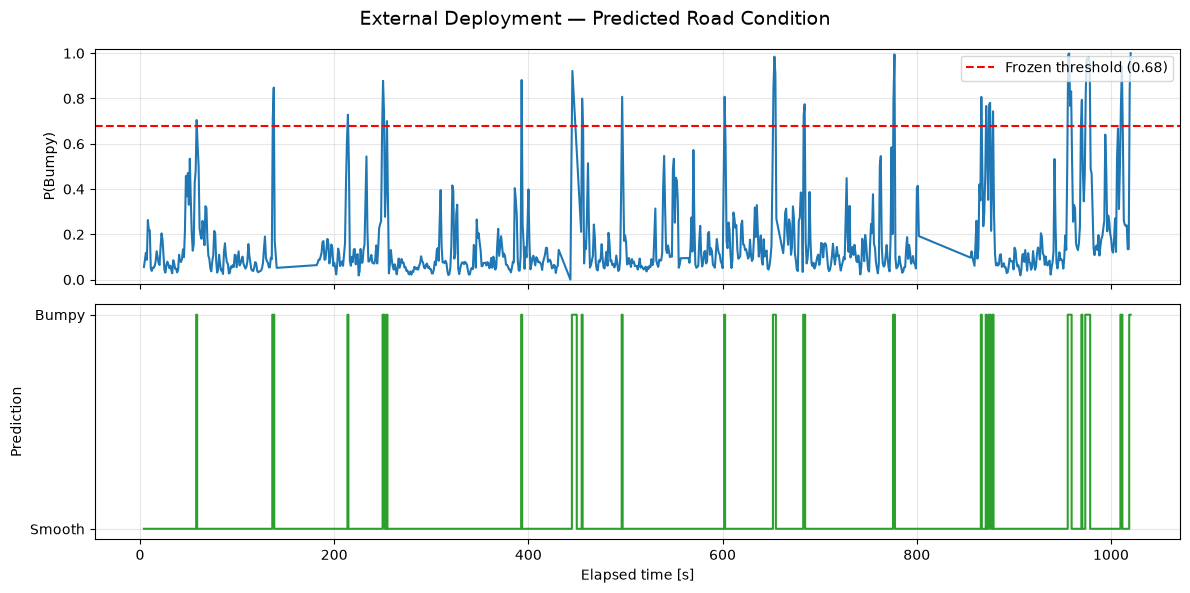
\includegraphics[width=0.9\linewidth]
    {figures/deployment-prediction.png}
    \caption{Deployment of the frozen Logistic Regression model on the
    independent external recording. The upper panel shows predicted Bumpy
    probability and the fixed threshold of 0.68; the lower panel shows the
    corresponding Smooth/Bumpy classification over elapsed time.}
    \label{fig:deployment-prediction}
\end{figure}

Because the external recording contains no terrain ground truth, these results
cannot be used to calculate classification performance. They instead
demonstrate that the complete preprocessing and inference pipeline can be
transferred to unseen sensor data and produce Smooth/Bumpy predictions over time, 
which would be suitable for a later stage real-time smartphone deployment.

\subsection{Limitations and Recommendations}

The main limitation is the small number of independent acquisition units.
Although 4246 valid windows were extracted, overlapping windows from the same
ride are correlated and should not be interpreted as independent experiments.
After participant~\#03 was excluded because of sampling-rate incompatibility,
only two participants remained.

The held-out results also indicate substantial recording-dependent
generalisation. In particular, the two unseen Bumpy recordings produced very
different outcomes: Raw022 achieved 87.5\% accuracy with mean Bumpy
probability 0.868, whereas Raw011 achieved only 11.6\% accuracy with mean
probability 0.414. Future data collection should therefore prioritise new
participants, devices, routes, riding speeds and acquisition sessions rather
than additional overlapping windows from existing rides.

A deployable implementation should also standardise a minimum sensor sampling
rate or redesign the spectral representation for devices unable to observe
the current 4--46~Hz band. Finally, the present preprocessing contains
offline/non-causal operations. Real-time smartphone deployment would require
causal filtering and explicit evaluation of latency, computational cost and
any resulting change in classification performance.

\clearpage
\printbibliography[heading=bibintoc,title={References}]

\clearpage
\begin{appendices}
\section{Empirical Measurements - Road Frequency versus Leg Movement Artifacts}

This appendix provides the raw experimental measurements supporting the
physics-informed frequency analysis summarized in
Section~\ref{sec:physics-eda}.

\begin{figure}[htbp]
    \centering
    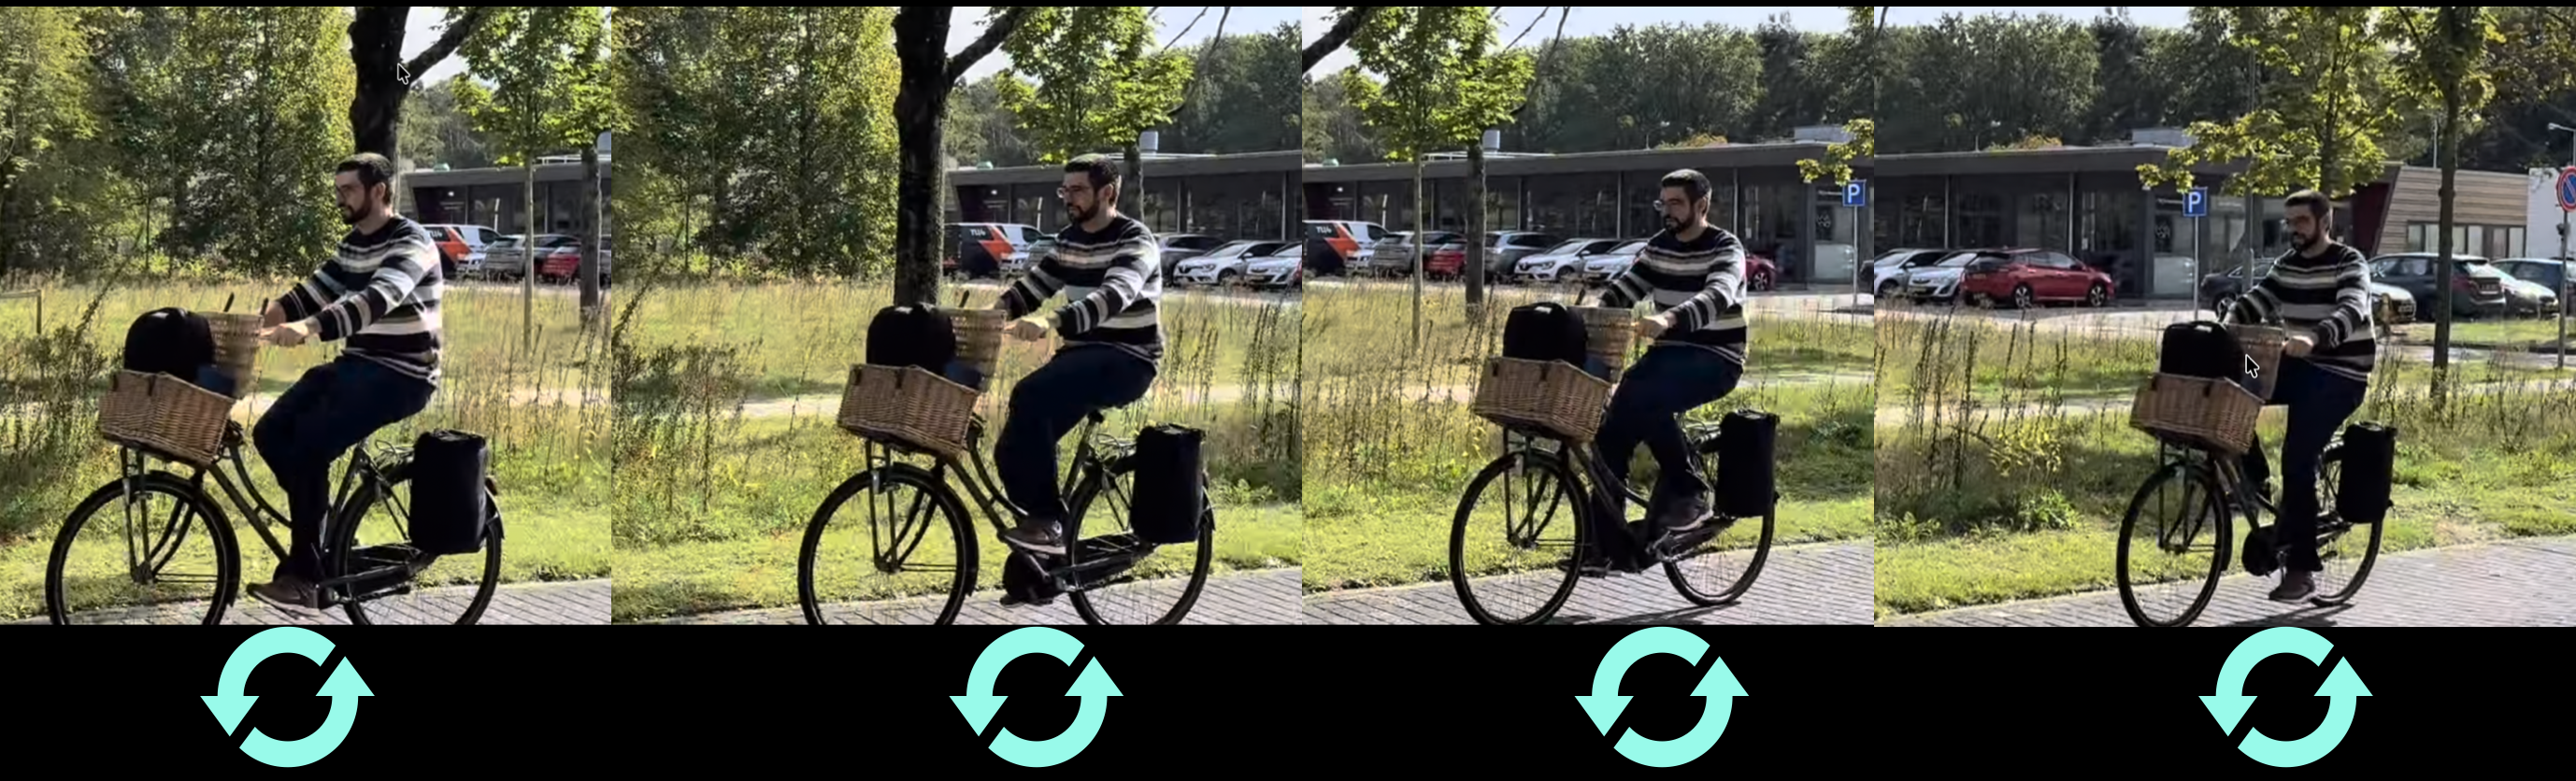
\includegraphics[width=0.8\linewidth]{figures/leg-movement}
    \caption{Example of manually counting the rotations per minute based on the video recording from one of the participants.}
    \label{fig:leg-mov}
\end{figure}

\begin{figure}[htbp]
    \centering
    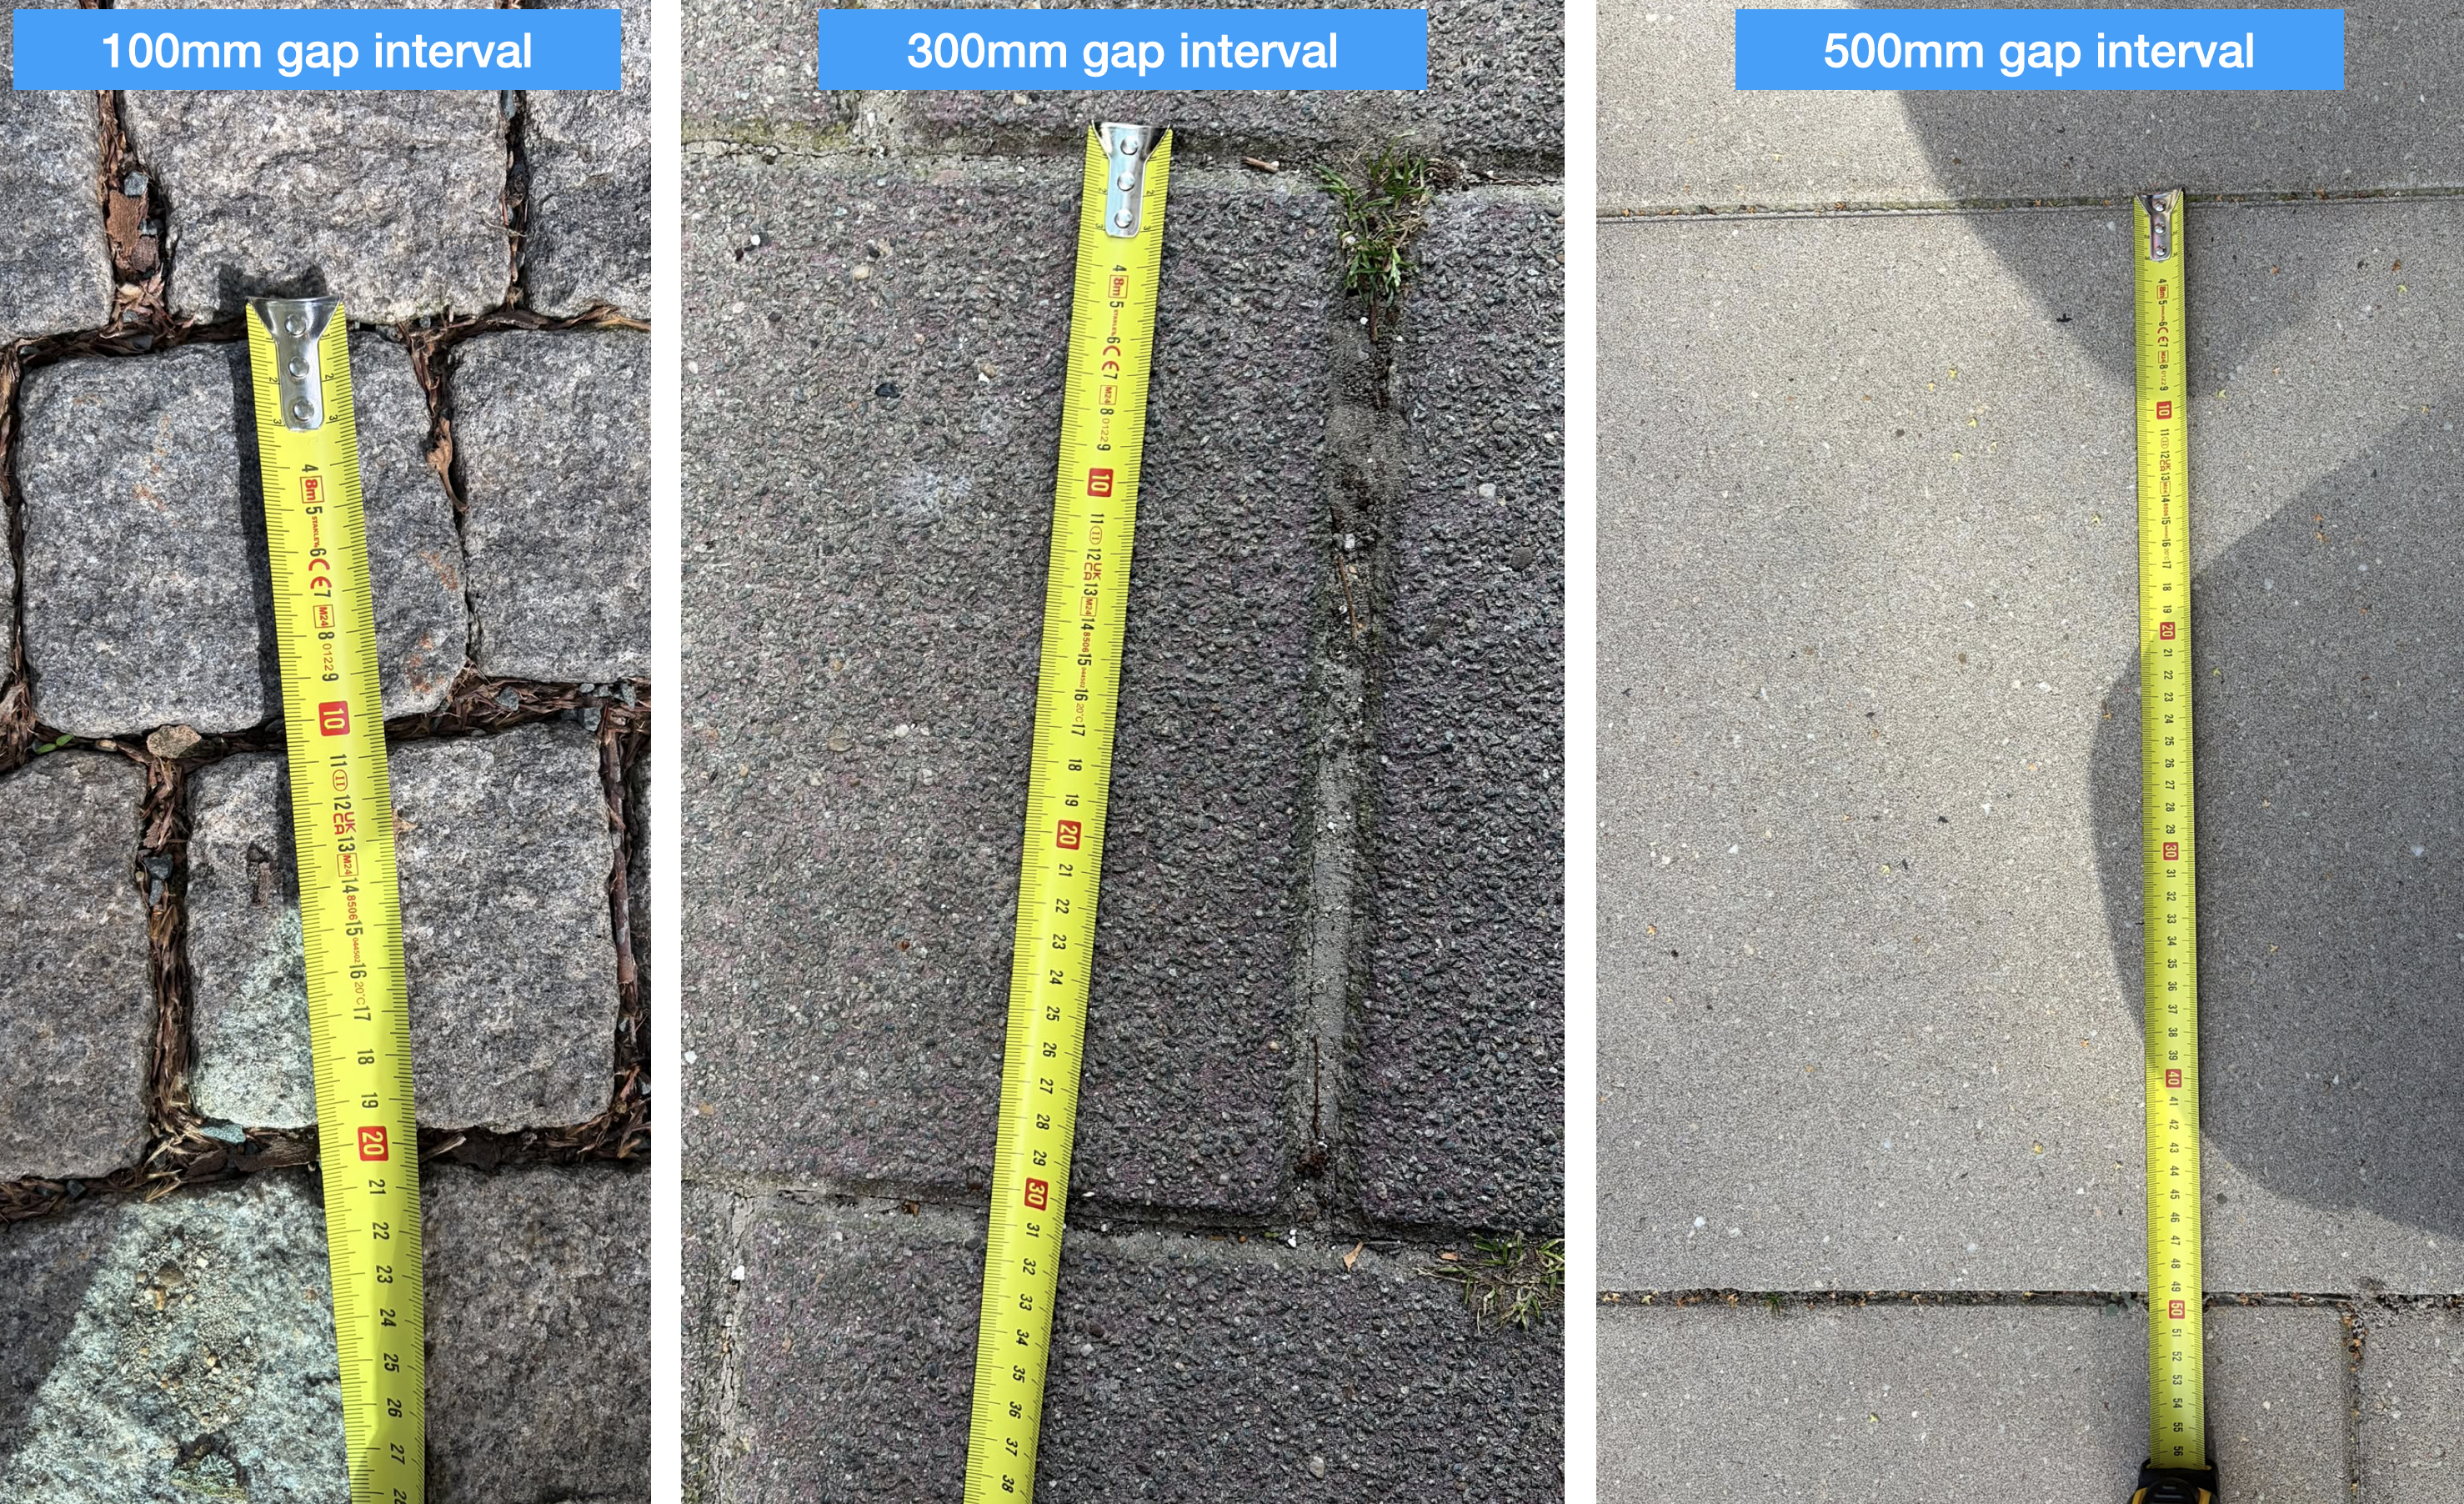
\includegraphics[width=0.8\linewidth]{figures/gap-bumpy-terrain}
    \caption{Different types of bumpy terrains were considered. The measured terrains ranged from $100 \sim 500mm$ gap interval.}
    \label{fig:road-gaps}
\end{figure}


\begin{table}[htbp]
    \centering
    \caption{Measured cycling speed and estimated road-excitation frequency for a terrain spacing of $\lambda = 100$ mm.}
    \label{tab:road_frequency}
    \begin{tabular}{ccccccccc}
        \toprule
        $\lambda$ 
        & Distance
        & Intended
        & $t_1$
        & $t_2$
        & $t_3$
        & $\bar{t}$
        & Speed
        & $f_{\text{road}}$ \\
        (mm)
        & (m)
        & speed
        & (s)
        & (s)
        & (s)
        & (s)
        & (m/s)
        & (Hz) \\
        \midrule
        100 & 10 & Slow   & 3.63 & 4.06 & 4.03 & 3.91 & 2.56 & 25.60 \\
        100 & 10 & Medium & 2.50 & 2.45 & 2.60 & 2.52 & 3.97 & 39.74 \\
        100 & 10 & Fast   & 1.95 & 1.85 & 2.06 & 1.95 & 5.12 & 51.19 \\
        \bottomrule
    \end{tabular}
    \label{tab:road-freq}
\end{table}


\begin{table}[htbp]
    \centering
    \caption{Estimated pedalling cadence from manually counted leg-motion cycles.}
    \label{tab:pedalling_frequency}
    \begin{tabular}{lcccc}
        \toprule
        Video
        & Duration
        & Cycles counted
        & $f_{\text{pedal}}$
        & Cadence \\
        & (s)
        &
        & (Hz)
        & (RPM) \\
        \midrule
        rpm-video-1.mp4 & 17 & 26 & 1.53 & 91.76 \\
        rpm-video-2.mp4 & 21 & 30 & 1.43 & 85.71 \\
        rpm-video-3.mp4 & 25 & 30 & 1.20 & 72.00 \\
        \bottomrule
    \end{tabular}
    \label{tab:leg-rpm}
\end{table} 

\section{Data Acquisition and Signal-Processing Diagnostics}
\label{app:data-diagnostics}

This appendix presents additional diagnostic evidence supporting the
data-quality screening, operational-state detection and physics-informed
signal-processing decisions described in Sections \ref{sec:data-understanding} and \ref{sec:data-preparation}.

\begin{figure}[p]
    \centering
    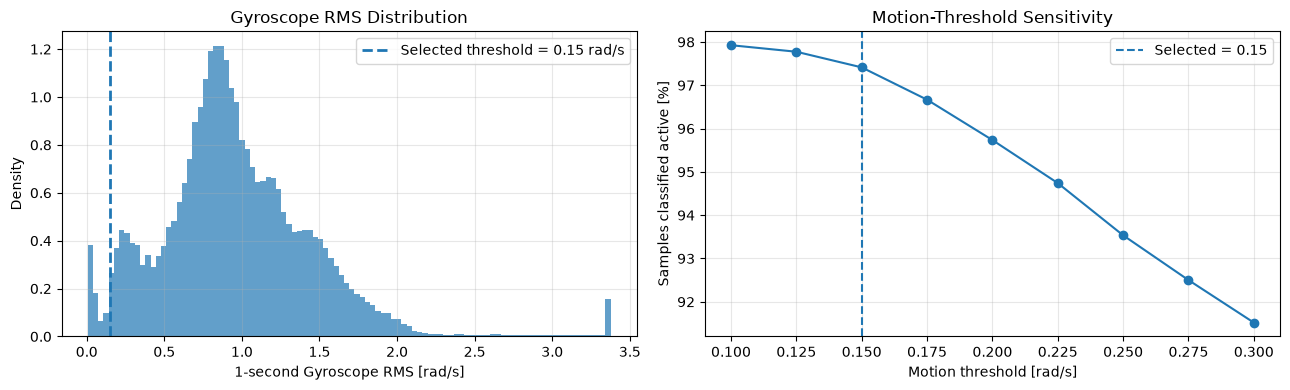
\includegraphics[width=\textwidth]
    {figures/motion-threshold-selection.png}
    \caption{Diagnostic analysis used to select the gyroscope-based motion
    threshold. The left panel shows the distribution of the one-second
    gyroscope RMS envelope and the selected threshold of 0.15~rad/s.
    The right panel shows the sensitivity of the proportion of samples
    classified as active to alternative threshold values.}
    \label{fig:appendix-motion-threshold}
\end{figure}



\begin{figure}[p]
    \centering
    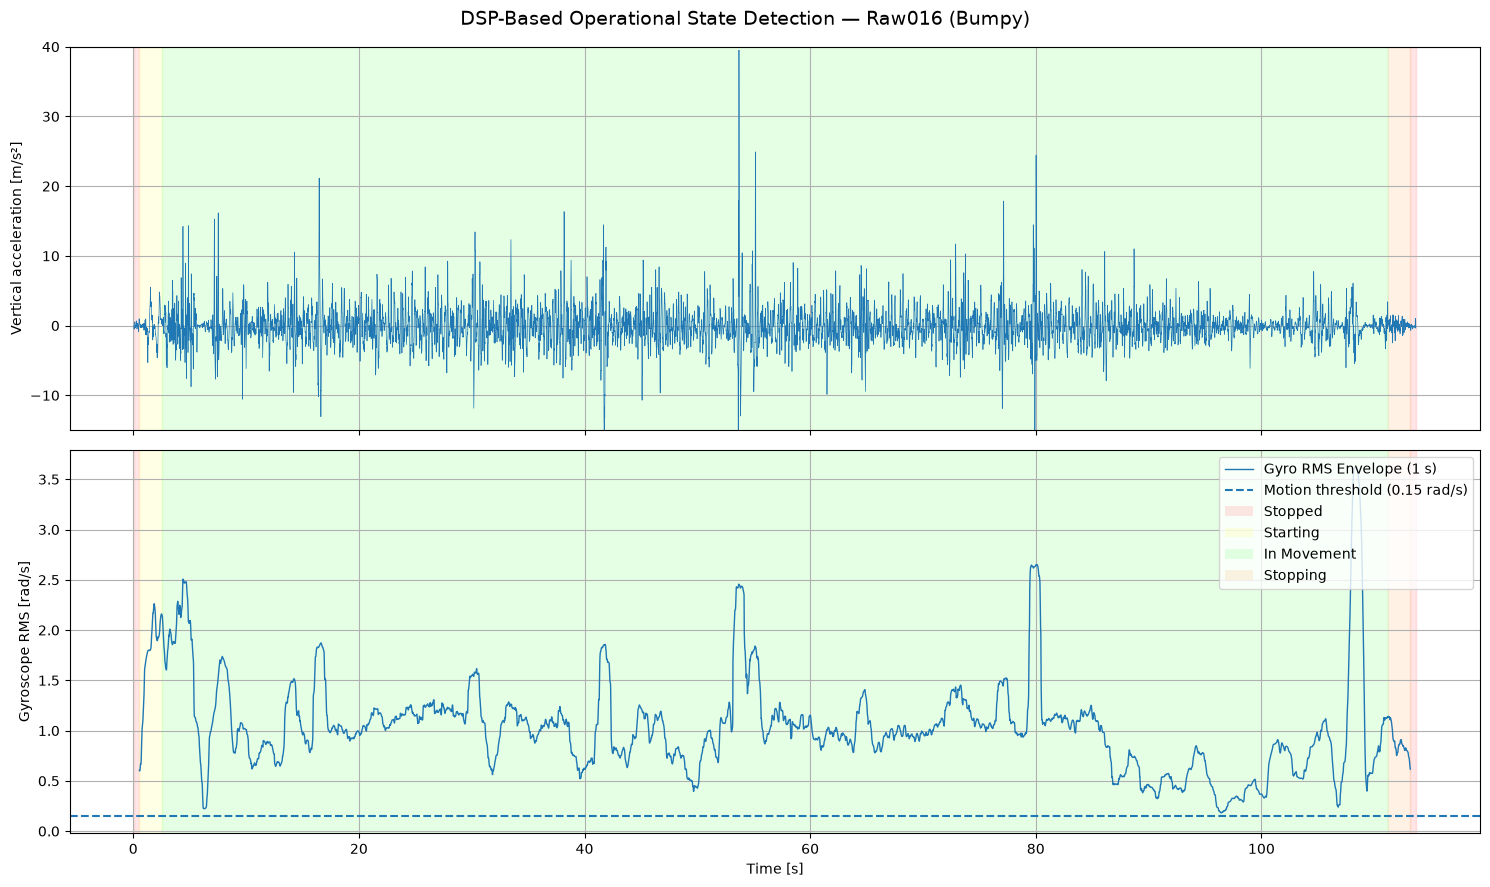
\includegraphics[width=\textwidth]
    {figures/dsp-based-state-detection-example.png}
    \caption{Example of DSP-based operational-state detection for a Bumpy
    recording. The upper panel shows vertical dynamic acceleration and the
    lower panel the smoothed gyroscope RMS envelope. Background shading marks
    samples classified as Stopped, Starting, In Movement and Stopping. Only
    stable In Movement regions were retained for feature extraction.}
    \label{fig:appendix-state-detection}
\end{figure}

\clearpage
\section{Model Validation Diagnostics}
\label{app:model-diagnostics}

This appendix provides the detailed confusion matrices corresponding to the
training-only supervised and unsupervised model comparisons discussed in
Section \ref{sec:evaluation}.

\subsection{Supervised out-of-fold comparison}

\begin{figure}[p]
    \centering
    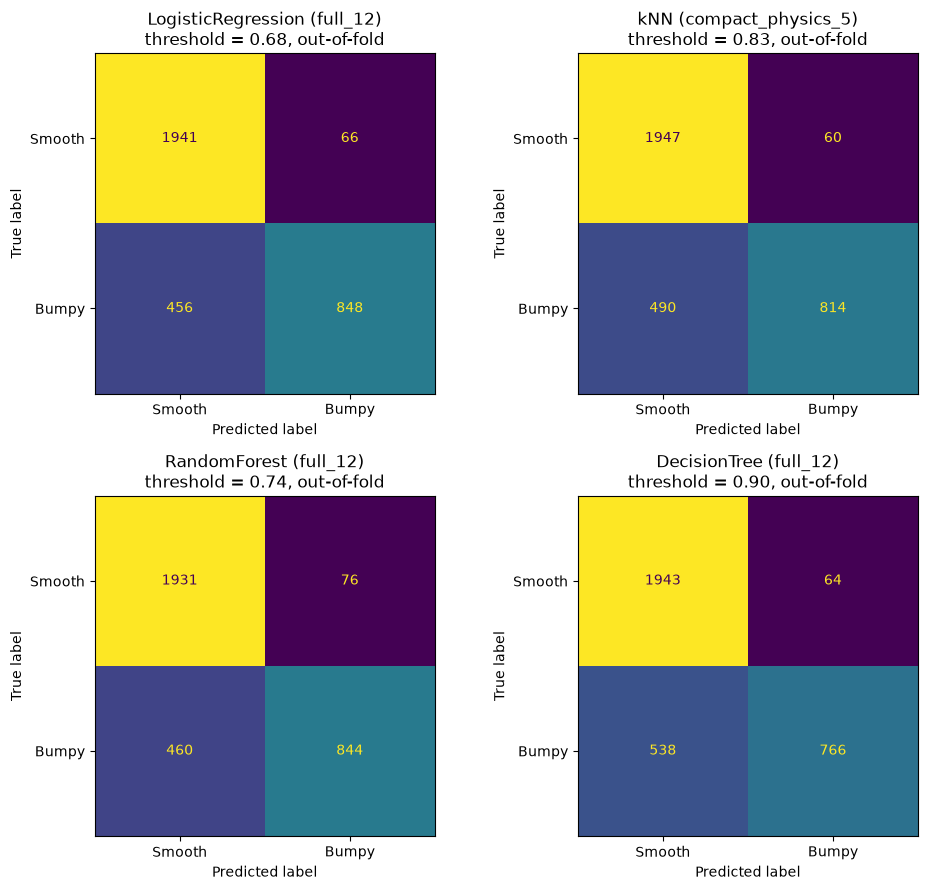
\includegraphics[width=\textwidth]
    {figures/confusion-matrices-supervised.png}
    \caption{Training-only out-of-fold confusion matrices for the best
    configuration from each supervised model family. The thresholds shown
    were selected using out-of-fold training predictions and were fixed before
    final held-out evaluation. Logistic Regression achieved the highest
    validation $F_{0.5}$ score and was therefore selected as the final model.}
    \label{fig:appendix-supervised-cm}
\end{figure}

Across the supervised candidates, all selected operating points favour a low
false-positive rate for Bumpy predictions. Logistic Regression provided the
best $F_{0.5}$ compromise, with 66 Smooth windows incorrectly classified as
Bumpy and 848 correctly detected Bumpy windows in the combined out-of-fold
training predictions.

\subsection{Unsupervised comparison}

\begin{figure}[p]
    \centering
    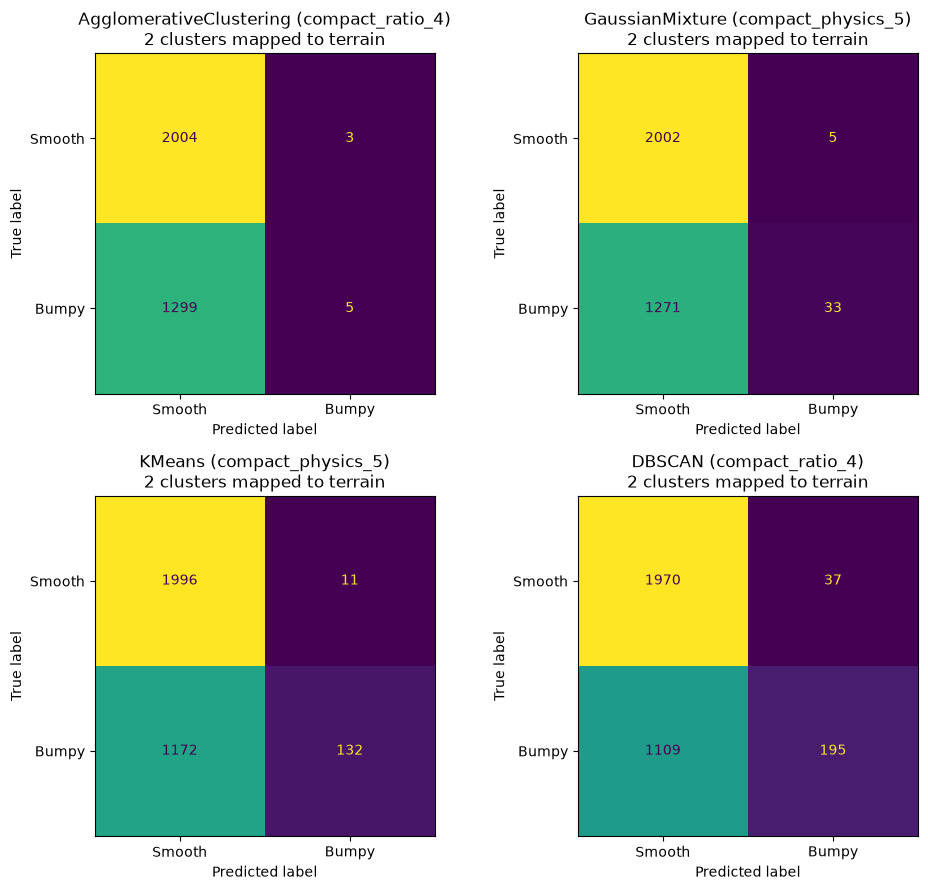
\includegraphics[width=\textwidth]
    {figures/confusion-matrices-UNsupervised.png}
    \caption{Mapped training-set confusion matrices for the best configuration
    from each unsupervised clustering family. Terrain labels were not used
    during clustering and were applied only afterwards to map clusters for
    diagnostic comparison.}
    \label{fig:appendix-unsupervised-cm}
\end{figure}

The mapped confusion matrices reinforce the distinction between internal
cluster separation and terrain-class agreement. Agglomerative Clustering and
Gaussian Mixture Modelling formed internally well-separated structures, but
these structures mapped predominantly to the Smooth class. DBSCAN produced
the greatest correspondence with the Smooth/Bumpy target among the evaluated
clustering methods, although its agreement remained weak compared with the
supervised approaches.



\end{appendices}

\end{document}
